\documentclass[11pt,a4paper]{article}

% Langue
\usepackage[french]{babel}
\usepackage[utf8]{inputenc}
\usepackage[T1]{fontenc}

% Mise en page
\usepackage[scale=0.7]{geometry}
% Pied de page
\usepackage{fancyhdr}
\pagestyle{fancy}
\renewcommand{\headrulewidth}{0pt}
\setlength{\headheight}{13.6pt}
% Interligne après les paragraphes
\setlength{\parskip}{5pt}

% Images
\usepackage{graphicx}
\usepackage{subcaption}
\usepackage{wrapfig}

% Rond plutôt que des tirets dans les listes
\renewcommand{\Frlabelitemi}{\textbullet}

% Bibliographie
\bibliographystyle{plain}
\usepackage{url}% Used for printing URL

\begin{document}

\newcommand{\HRule}{\rule{\linewidth}{0.5mm}}

\begin{titlepage}
\begin{center}


\includegraphics[width=0.5\textwidth]{polytech}~\\[1cm]

\textsc{\LARGE EISD}\\[1.5cm]

\textsc{\Large Extraction d'information et Système de dialogue}\\[0.5cm]

% Title
\HRule \\[0.4cm]
{ \huge \bfseries Création d'un système de dialogue complet\\ [0.4cm] }
\HRule \\[1.5cm]

% Author and supervisor
\begin{minipage}{0.4\textwidth}
\begin{flushleft} \large
\emph{Auteurs:}\\
Romain \textsc{Jayez}\\
Guillaume \textsc{Monnet}
\end{flushleft}
\end{minipage}
\begin{minipage}{0.4\textwidth}
\begin{flushright} \large
\emph{} \\
Steven \textsc{Nabbs}\\
Luc \textsc{Poncet}
\end{flushright}
\end{minipage}

\vfill

% Bottom of the page
{\large \today}

\end{center}
\end{titlepage}


\rhead{EISD - Rapport}
\lfoot{
\includegraphics[scale=0.3]{polytech.jpg}}
\rfoot{JAYEZ - MONNET \\ NABBS - PONCET}

\tableofcontents

\clearpage

\section{Introduction}
%Schema du systéme ?

Le but du projet est de créer un système permettant d'engager un dialogue question-réponse avec un utilisateur. Le système répond en puisant les informations dans une base de données. Cette base à été préalablement remplis grâce à des informations extraites depuis différents éléments comme des texte, tableaux et ceci provenant de toute sources disponibles. 
La circulation des données est illustrée par la figure \ref{fig:schema} en dessous.

\begin{figure}[!htb]
	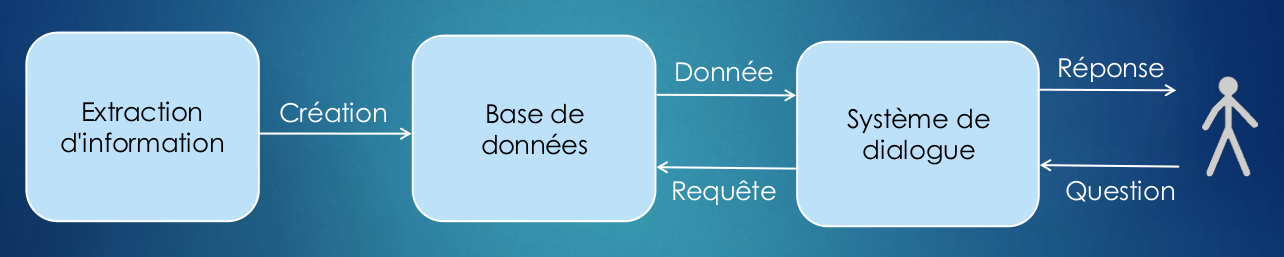
\includegraphics[width=\textwidth]{schemaSysteme.png}
	\caption{Schèma simplifié du fonctionnement de système}
	\label{fig:schema}
\end{figure}

Des systèmes équivalent de grandes ampleurs sont déjà utilisés tous les jours. Pour ce projet, il est demandé de réaliser un version minimaliste avec des informations concentrés sur un seul sujet.

Il existe plusieurs manière de récupérer et remplir une base de données, les principales sont de récupérer directement les informations depuis un tableau, c'est la manière la plus rapide, la plus simple, et on obtient une grande masse de données. Ensuite extraire l'information depuis des textes, pour cela il faut établir des listes de règles et des expression régulière pour récupérer l'information. Cette méthode est donc plus compliqué à mettre en place, mais cela permets toujours d'automatiser la récupération de l'information. Ensuite quand les informations sont ne sont pas récupérable par les méthodes précédente, il est plus rentable d'ajouter manuellement une information dans la base de données que de créer une règle spécifique.
Dans le projet on utilise la méthode d'extraction d'information dans les textes pour remplir de la base. Cela nous permets d'être confronté aux problèmes que pose la rédaction des règles.

Deux sujets était proposés, le premier, des descriptions provenant du site Wikipédia d'un grand nombre de pays. Le second, des recettes et commentaires issues du site Marmiton. Nous avons choisis les descriptions des pays pour la propreté de rédaction des textes.

Le projet est réaliser en langage lua, langage de script léger et performant. On utilise un programme nommé dark qui est un outils de développement pour la création des règles. Celle-ci s'utilise de la même manière que des expressions régulières. L'outil permet également l'application de tag dans les textes et une sérialisation de tableau pour remplir la base de données faite en lua. 


\clearpage

\section{Extraction d'information}

\subsection{Composition de la base de données}

Pour démarrer, nous avons regardé une certaine quantité de description sur les pays et nous avons repéré les informations récurrente dans chaque fichier. Avec ceci nous avons crée la base fictive contenant chaque type d'information que l'on aimerait récupérer.

Choix initial des informations à récupérer :
\begin{itemize}
	\item Capitales
	\item Pays Frontaliers
	\item Monnaie
	\item Continent
	\item Religions
	\item Population
	\item Régime
	\item Superficie
	\item Position (GPS, etc.)
\end{itemize}

L'information Position devait contenir une position GPS, ou tout autre élément permettant de situer le pays. Or la position GPS n'est pas présente dans les différents textes et la position est déjà donnée grâce aux informations Continent et Pays Frontaliers. Donc nous avons retirer l'information Position de notre base de données.


\subsection{Les problèmes rencontrés}
Pas de formatage des informations
Création empirique des patterns
Erreurs lié à dark (ex: nom propre parfois reconnu comme adjectif)
Récupération des tags pour la base de donnée

Initialement « façon xml » puis utilisation des fonctions fournies (+ variantes
personnelles)
Gestion de la ponctuation, majuscules/minuscules
Choix de listes fermées/ouvertes ?

\subsection{La couverture d'information de la base}
Nous avons réaliser un script permettant de calculer le rapport d'information présente dans la base de données par rapport au nombre total de pays.

Voici les résultats (arrondi au \%) après avoir effectué les dernières modifications sur nos règles :
% bla bla completage
\begin{itemize}
	\item Langue 		  : 22\%
	\item Continent 	  : 84\%
	\item Capitale 		  : 38\%
	\item Pays Frontalier : 43\%
	\item Superficie	  : 21\%
	\item Population 	  : 38\%
	\item Régime 		  : 9\%
	\item Religion		  : 12\%
	\item Monnaie		  : 22\%
\end{itemize}

  


\subsection{Améliorations possibles}
Vérifications de la qualité des informations dans la base de données :
Par exemple, la liste des pays frontalier d'un pays X, on peut vérifier que chaque pays contenu dans la liste, a bien le pays X comme pays frontalier.

\clearpage

\section{Système de dialogue}

\subsection{Les questions}

Nous avons choisi de parser la question et de nous arrêter à la lecture du point d’exclamation. Tout ce qui suit le ‘ ?’ n’est pas pris en compte. Cela nous permet d’éviter de devoir traiter plusieurs questions en même temps. Si l’utilisateur ne rentre pas de point d’exclamation la question n’est pas reconnue comme telle et nous n’y donnons donc pas suite.
 
Le but de la reconnaissance d’informations est de taguer les informations essentielles dans la question, à savoir le contexte et le sujet. Le contexte ici étant le pays, et le sujet étant les informations importantes le concernant. Ces informations sont les suivantes :
Capitale
Monnaie
Continent
Religion
…


Nous avons choisi de stocker la réponse à ces informations de la sorte :
France {
            	monnaie = ‘’,
            	capitale = ‘Paris’,
            	religions = {},
            	pays\_frontaliers = { Espagne, Allemagne, Suisse }
}
Soit un champ est vide, soit il contient une valeur, ou soit il contient un tableau de valeurs (qui peut être vide également).
 
 
Récupérer le sujet/thème de la question (capitale, monnaie, pays voisins, religion,) et récupérer le contexte/pays sur lequel la question porte.
« Quelle est la capitale de la France ? » 
 
Prendre en compte le fait qu’il puisse y avoir plusieurs sujets pour une question.
« Quelles sont les capitales de l’Afrique du Sud et sa devise ? »
 
Prendre en compte le fait qu’il puisse y avoir plusieurs contextes pour une question.
« Quelle est la capitale de la France et celles de l’Afrique du Sud ? »
 
Gérer l’historique pour un ou plusieurs contextes.
« Quelle est la capitale de l’Espagne et de la France ? »
« Et leur monnaie ? »
 
Gérer l’historique pour un ou plusieurs sujets.
« Quelle est la devise de la Belgique et ses religions ? »
« Et pour la France ? »
 
Ajout d’une table de jointure pour trouver si 2 pays ont des contextes en commun (ajout d’un tag sur les mots en commun). Renvoie tous les pays frontaliers en commun entre 2 pays :
« Quels sont les pays voisins en commun entre la France et l’Autriche ? »
 
Renvoie tous les pays frontaliers en commun entre les 3 pays et renvoie ceux en commun entre 2 pays deux à deux avec un pourcentage d’intersection :
« Quels sont les pays voisins en commun entre la France et l’Autriche et l’Espagne ? »
 
 
Nous nous sommes ensuite intéressés au fait de répondre à des interrogations faites directement sur la base de données. Nous avons donc choisi de taguer le mot « base ». Et donc les questions suivantes renvoient toute une réponse pertinente.
 
Interrogation sur un ou plusieurs pays dans base renvoie de façon structurée toutes les informations le(s) concernant
« Quelles sont les données en base que tu possèdes sur la France et l’Espagne ? »
 
Interrogation sur un ou plusieurs sujets dans la base de données renvoie toutes les informations, sans doublons, disponibles et présentes pour chaque pays.
« Quelles sont les devises et les religions présentes en base ? »
 
 
 
 
Corriger la synthaxe
 
France Espagne base
France Espagne monnaie base => question classique
Monnaie base => toutes les monnaies de la base  (donner d’abord le nombre de réponse, puis proposer à l’utilisateur de les afficher)
Pays en afrique =>
 
Nous avons pensé à poser une question du type : «  Quels sont tous les pays dans la base de données qui possèdent l’euro ?». Pour répondre à cette question nous aurions pu parcourir la base jusqu’à atteindre le mot « euro » une première fois puis  récupérer le tag « monnaie » associé à ce mot. Enfin nous aurions récupéré tous les pays dont le tag « monnaie » contiendrait « euro ». Mais finalement, nous avons conclu que cela ne pourrait marcher que pour une petite base de données donc nous avons choisi de ne pas implémenter ce type de réponse. 


\section{Conclusion}

Ce projet nous a permis d'appréhender le langage Lua. Ce langage se révèle être capable de faire des scripts léger et puissant. Il est justement apprécié dans le milieu professionnel pour ses qualités, et même très présent dans le milieu du jeu vidéo. L'apprentissage de ce langage pourra se montrer utile par la suite.

\end{document}
